% kapitel5.tex
\chapter{Optimization Studies for the Event Selection}

\section{Search for Discriminating Variables }
\label{distributions}
The first part of the optimization studies is the search for variables which provide a significant distinction between background and signal.
Caused by the basic selection discussed in section \ref{basic selection} already much background is rejected.
Moreover, the requirement of two large-R jets, which fulfill the minimum criteria (Table \ref{calibration}, cause that the remaining background events have high momenta.
Therefore the background is also expected in the high energy regions, which is also expeced for the signal processes.\\
%This complicates the search for discriminating variables, because the signal is expected to contain high energies,too.\\
Figure \ref{H_T} shows the distribution for the scalar sum of the transverse momenta of all jets in an event.

\begin{figure}
\centering
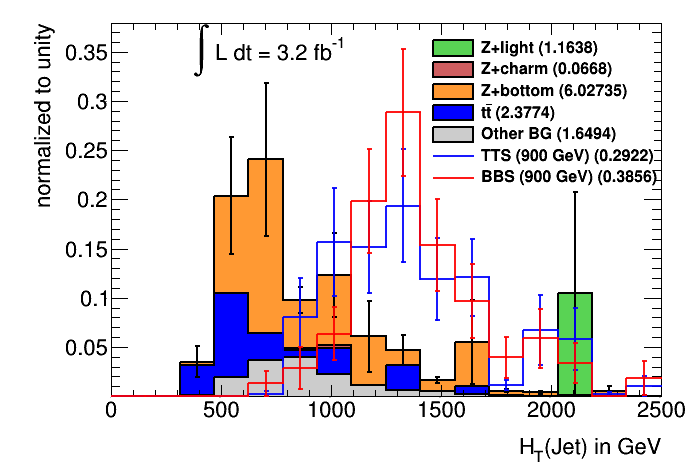
\includegraphics[width=8cm]{figures/H_T.png}
\caption{Distribution of the scalar sum of all jet $p_{T}$'s in an event after the preselection. 
Both signal and background are presented and the distributions are normalized to unity. 
The number of events, displayed in brackets, is expected for an integrated luminosity $\int L dt$ = \SI{3.2}{fb^{-1}.}
The vertical lines represent the statistical uncertainties.}
\label{H_T}
\end{figure}

The distribution shows that the signal is shifted to the right compared to the background, because there are higher momenta in the events resulting from the very massive vector-like quarks.
There are also much background events, relative to the total amount of background events, in the signal region, which is as expected, because of the requirements of the basic selection. \\
Figure \ref{Zpt} presents the distribution of the Z candidate $p_{T}$, which in the following is denoted as $p_{T}(Z)$.
\begin{figure}
\centering
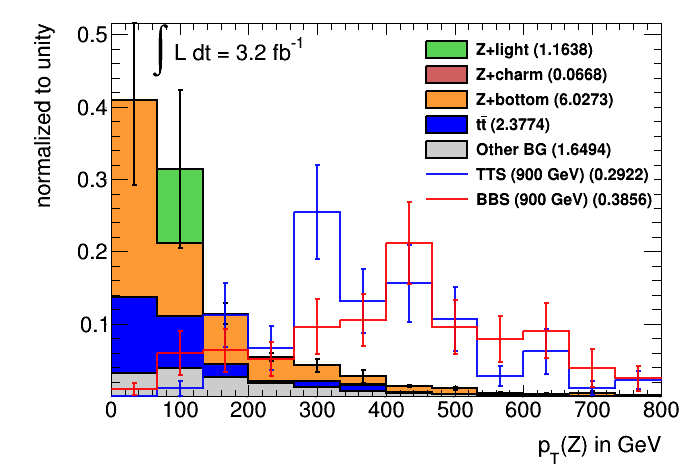
\includegraphics[width=8cm]{figures/Zpt.png}
\caption{$p_{T}(Z)$ distribution for signal and background after the preselection. 
Both signal and background are normalized to unity.  
The number of events, displayed in brackets, is expected for an integrated luminosity $\int L dt$ = \SI{3.2}{fb^{-1}.}
The vertical lines represent the statistical uncertainties.}
\label{Zpt}
\end{figure}

As mentioned for the $H_{T}$ distribution the signal is shifted to the right. That is expected, because the Z boson results straight from the vector-like quark and has a momentum $p$ about \SI{450}{GeV}.\\
In figure \ref{leadingljet} the $p_{T}$ of the large-R jet with the highest $p_{T}$ of an event is represented, which in the following is denoted as $p_{T}(leading large-R jet)$.
\vspace{-0.5cm}
\begin{figure}[h!]
\centering
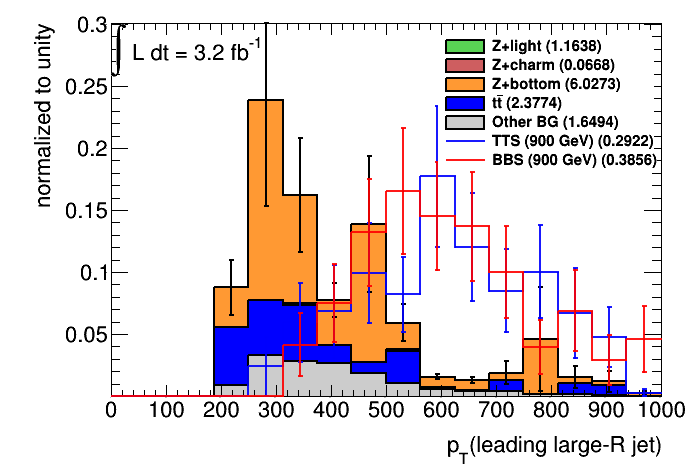
\includegraphics[width=8cm]{figures/leadingljet.png}
\caption{Distribution of $p_{T}(leading large-R jet)$ for signal and background after the preselection. 
Both signal and background are normalized to unity.  
The number of events, displayed in brackets, is expected for an integrated luminosity $\int L dt$ = \SI{3.2}{fb^{-1}.}
The vertical lines represent the statistical uncertainties.}
\label{leadingljet}
\end{figure}

It is visible that the signal has higher values for $p_{T}(leading large-R jet)$ than the background.
The large-R jet with the highest $p_{T}$ is expected to cluster the decay products of the top quark or W boson resulting from the vector-like quark decay.
Therefore a high momentum is expected for the leading large-R jets of the signal processes.\\
Figure \ref{mZbdist} shows the distribution of the invariant mass of the Z candidate and the highest $p_{T}$ b-jet $m(Zb)$ and \ref{mZtdist} the invariant mass of the Z candidate and the highest $p_{T}$ top-jet $m(Zt)$.


%\resizebox{0.48\columnwidth}{!}{
\begin{figure}[h]
    \centering
    \resizebox{0.46\columnwidth}{!}{
    \begin{subfigure}{.49\textwidth}
      \centering
      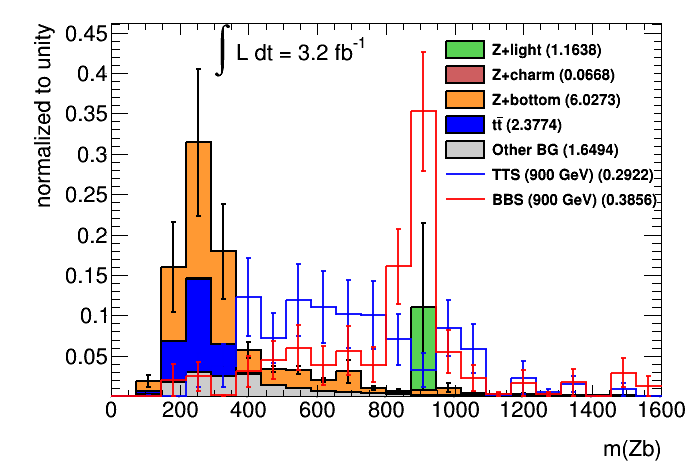
\includegraphics[width=.99\linewidth]{figures/mZb.png}
      \caption{}
      \label{mZbdist}
    \end{subfigure}
    }
    \resizebox{0.46\columnwidth}{!}{
    \begin{subfigure}{.49\textwidth}
      \centering
      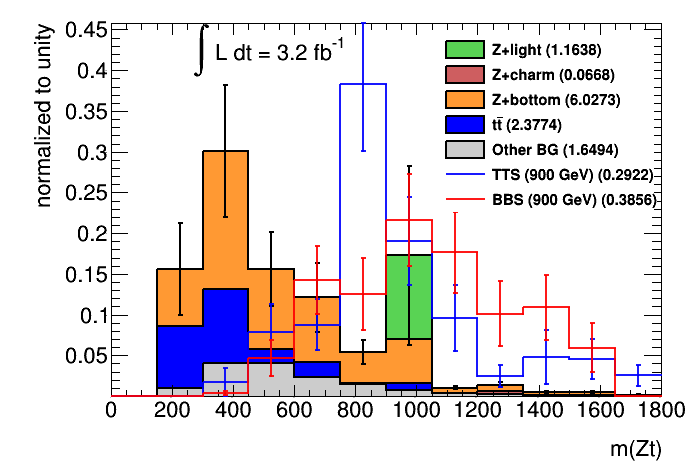
\includegraphics[width=.99\linewidth]{figures/mZt.png}
      \caption{}
      \label{mZtdist}
    \end{subfigure}
    }
    \caption{Plot for (a) the invariant mass of the Z candidate and the highest $p_{T}$ b-jet and (b) the invariant mass of the Z candidate and the highest $p_{T}$ top-jet . 
Both signal and background are presented and the distributions are normalized to unity. 
The number of events, displayed in brackets, is expected for an integrated luminosity $\int L dt$ = \SI{3.2}{fb^{-1}.}
The vertical lines represent the statistical uncertainties.}
    \label{mZb+mZt}   
\end{figure}
%}
The signal is shifted to the right, because the Z candidate and both the b-jet and top-jet are expected to have high momenta, which is shown in the previous distributions. 
For the BBS signal process there is a peak at \SI{900}{GeV} in figure \ref{mZbdist} and for the TTS signal process in figure \ref{mZtdist}.
This is as expected because the Z candidate and the highest $p_{T}$ b-jet respectively top-jet result from the vector-like quark decay B \texorpdfstring{$\longrightarrow$}~Zb or T \texorpdfstring{$\longrightarrow$}~Zt and the vector-like quark masses are simulated with $m_{T,B}$ = \SI{900}{GeV} .\\
Generally, the presented distributions provide the possibility to achieve a distinction between background and signal by requiring limits for different variables.


\section{Significance for Different Cuts}
\label{optimization}
In this section the significance for different limits on variables, which are shown in section \ref{distributions}, are examined.
In a previous search for vector-like quarks with a center of mass energy $\sqrt{s}$ = \SI{8}{TeV} \cite{8tevanalysis}, in the optimization studies $m(Zb)$ is chosen as final discriminant for the BBS and TTS process .
In this analysis $m(Zb)$ is chosen as final discriminant for the BBS process,too, but $m(Zt)$ is chosen separately for the TTS process.
The boosted analysis provides the possibility of this variable by using top tagging.
The optimization studies are performed with an interval of the distributions of the final discriminants.
The interval is chosen, so that 80\% of all signal events of BBS respectively TTS are within the interval starting from the highest values of $m(Zb)$ or $m(Zt)$. 
This interval is chosen because the signal is shifted to higher values of $m(Zb)$ and $m(Zt)$ compared to the background.
Therefore in the interval the main background is rejected. 
The significance of the signal relative to the fluctuations of the background is investigated with formula $\frac{s}{\sqrt{b}}$, while $\sqrt{b}$ describes the statistical uncertainty of the background and $s$ the number of signal events.
For both s and b the weighted number of events is considered.\\
Figure \ref{mZbcut} shows the significance as function of varying limits considering the variables presented in section \ref{distributions} for the chosen interval of $m(Zb)$. 



\begin{figure}[h]
    \centering
    \resizebox{0.46\columnwidth}{!}{
    \begin{subfigure}{.49\textwidth}
      \centering
      \includegraphics[width=.99\linewidth]{figures/H_TcutmZb.pdf}
      \caption{}
      \label{HTmZb}
    \end{subfigure}
    }
    \centering
    \resizebox{0.46\columnwidth}{!}{
    \begin{subfigure}{.49\textwidth}
      \centering
      \includegraphics[width=.99\linewidth]{figures/leadingljetptcutmZb.pdf}
      \caption{}
      \label{ljetmZb}
    \end{subfigure}
    }
    \centering
    \resizebox{0.46\columnwidth}{!}{
    \begin{subfigure}{.49\textwidth}
      \centering
      \includegraphics[width=.99\linewidth]{figures/ZptcutmZb.pdf}
      \caption{}
      \label{ZpTmZb}
    \end{subfigure}
    }
    \caption{Distribution for the significance for m(Zb) as function of varying limits for (a) $H_{T}$ , (b) leading large-R jet $p_{T}$ and (c) Z boson $p_{T}$.
    The cut values varying with \SI{50}{GeV} steps.
    The significance is calculated for interval of m(Zb), which starts with the highest value of m(Zb) and ends if 80 \% of the total number of BBS signal events are within the interval.}
    \label{mZbcut}   
\end{figure}
    

The graphs are consistent with the trends of the distributions presented in section \ref{distributions}.
For $H_{T}$ and leading large-R jet $p_{T}$ the significance has higher values for lower limits and decreases fastly for higher limits.
This is expected, because the signal distribution is only slightly shifted to higher values and therefore for higher limits the peak of the signal is rejected.
The significance is proportional to the absolute number of signal events, therefore lower values are expected if a lot of signal is rejected.\\
For the $p_{T}(Z)$ distribution the signal shift is more distinct.
Therefore higher limits can be set to reject a lot of background and still not cut into the main signal region.
The significance has lower values for lower limits, because there is not much background rejected, and it increases, if the main background is rejected but not the signal and finally decreases when big parts of the signal are discarded.\\
Figure \ref{mZtcut} shows the significance as function of varying limits considering the variables presented in section \ref{distributions} for the chosen interval of $m(Zt)$.


\begin{figure}[h!]
    \centering
    \resizebox{0.46\columnwidth}{!}{
    \begin{subfigure}{.49\textwidth}
      \centering
      \includegraphics[width=.99\linewidth]{figures/H_TcutmZt.pdf}
      \caption{}
      \label{HTmZt}
    \end{subfigure}
    }
    \centering
    \resizebox{0.46\columnwidth}{!}{
    \begin{subfigure}{.49\textwidth}
      \centering
      \includegraphics[width=.99\linewidth]{figures/leadingljetptcutmZt.pdf}
      \caption{}
      \label{ljetmZt}
    \end{subfigure}
    }
    \centering
    \resizebox{0.46\columnwidth}{!}{
    \begin{subfigure}{.49\textwidth}
      \centering
      \includegraphics[width=.99\linewidth]{figures/ZptcutmZt.pdf}
      \caption{}
      \label{ZpTmZt}
    \end{subfigure}
    }
    \caption{Distribution for the significance for m(Zt) as function of varying limits for (a) $H_{T}$ , (b) leading large-R jet $p_{T}$ and (c) Z boson $p_{T}$.
    The cut values varying with \SI{50}{GeV} steps.
    The significance is calculated for interval of m(Zt), which starts with the highest value of m(Zt) and ends if 80 \% of the total number of BBS signal events are within the interval.}
    \label{mZtcut}   
\end{figure}
    


The absolute value of the significance for the BBS process is higher, because there is a lower number of events for the TTS process.
The TTS distribution in figure \ref{Zpt} is shifted to lower values compared to the BBS distribution. 
Therefore it is as expected that the maximum of the significance for TTS is reached for lower limits than for the BBS signal process.
Figure \ref{HTmZb} and \ref{HTmZt} confirm the argumentation mentioned before.
The trends for leading large-R jet $p_{T}$ and $H_{T}$ can be explained with the same argumentation used for the BBS signal process.\\ 
Considering the plots for $p_{T}(leading large-R jet)$, $p_{T}(Z)$ and $H_{T}$ limits, the significance for the $p_{T}(Z)$ limits increases for both $m(Zt)$ and $m(Zb)$ to the highest values.  
Therefore the first limit is set for $p_{T}(Z)$.
The limit for both TTS and BBS are chosen to reach the highest value of $\frac{s}{\sqrt{b}}$.
Thereby the resulting limits are $p_{T}(Z) \geq$ \SI{250}{GeV} for TTS and $p_{T}(Z) \geq$ \SI{450}{GeV} for BBS. \\
In the following the significance as function of different limit for $p_{T}(leading large-R jet)$ and $H_{T}$, after requiring the $p_{T}(Z)$ limits, is investigated.
Figure \ref{mZbcutafterZpt} shows the significance for the $m(Zb)$ interval as function of varying limits, considering $H_{T}$ and leading large-R jet $p_{T}$, after the Z candidate $p_{T}$ limit is set.
Figure \ref{mZtcutafterZpt} represents the same varying limits for $m(Zt)$.

\begin{figure}[h]
    \centering
    \resizebox{0.46\columnwidth}{!}{
    \begin{subfigure}{.49\textwidth}
      \centering
      \includegraphics[width=.99\linewidth]{figures/H_TcutmZbafterZpt.pdf}
      \caption{}
      \label{HTmZbafterZpt}
    \end{subfigure}
    }
    \resizebox{0.46\columnwidth}{!}{
    \begin{subfigure}{.49\textwidth}
      \centering
      \includegraphics[width=.99\linewidth]{figures/leadingljetptcutmZbafterZpt.pdf}
      \caption{}
      \label{ljetmZbafterZpt}
    \end{subfigure}
    }
    \caption{Plot for the significance for $m(Zb)$ as function of varying limits for (a) $H_{T}$ , leading large-R jet (b)  $p_{T}$ after requiring $p_{T} \geq$ \SI{450}{GeV}.
    The values of the limits varying with \SI{50}{GeV} steps..
    The significance is calculated for interval of m(Zb), which starts with the highest value of m(Zb) and ends if 80 \% of the total number of BBS signal events are within the interval.}
    \label{mZbcutafterZpt}   
\end{figure}


\begin{figure}[h]
    \centering
    \resizebox{0.46\columnwidth}{!}{
    \begin{subfigure}{.49\textwidth}
      \centering
      \includegraphics[width=.99\linewidth]{figures/H_TcutmZtafterZpt.pdf}
      \caption{}
      \label{HTmZtafterZpt}
    \end{subfigure}
    }
    \resizebox{0.46\columnwidth}{!}{
    \begin{subfigure}{.49\textwidth}
      \centering
      \includegraphics[width=.99\linewidth]{figures/leadingljetptcutmZtafterZpt.pdf}
      \caption{}
      \label{ljetmZtafterZpt}
    \end{subfigure}
    }
    \caption{Plot for the significance for m(Zt) as function of varying limits for (a) $H_{T}$ ,(b) leading large-R jet $p_{T}$  after requiring $p_{T} \geq$ \SI{250}{GeV}.
    The values of the limits varying with \SI{50}{GeV} steps for $H_{T}$ and leading large-R jet $p_{T}$.
    The significance is calculated for interval of m(Zt), which starts with the highest value of m(Zt) and ends if 80 \% of the total number of BBS signal events are within the interval.}
    \label{mZtcutafterZpt}   
\end{figure}

For both TTS and BBS the $H_{T}$ limit distribution reaches a higher significance than the significance distribution for  $p_{T}(leading large-R jet)$.
The limit $H_ {T} \geq =$ \SI{1150}{GeV} provides the best significance for both TTS and BBS.\\
In the following it is examined, whether a further limit for $p_{T}(leading large-R jet)$, after requiring a Z candidate $p_{T}$ and $H_{T}$ limit, lead to an increasing significance.
Figure \ref{ljetptcutafterZptHT} shows the significance as function of varying leading large-R jet $p_{T}$ after the limits for Z candidate $p_{T}$ and $H_{T}$ limit are set.

\begin{figure}[h]
    \centering
    \resizebox{0.46\columnwidth}{!}{
    \begin{subfigure}{.49\textwidth}
      \centering
      \includegraphics[width=.99\linewidth]{figures/ljetcutafterZptHTmZb.pdf}
      \caption{}
      \label{HTmZtafterZptmZb}
    \end{subfigure}
    }
    \resizebox{0.46\columnwidth}{!}{
    \begin{subfigure}{.49\textwidth}
      \centering
      \includegraphics[width=.99\linewidth]{figures/ljetptcutafterZptHTmZt.pdf}
      \caption{}
      \label{ljetptcutafterZptmZt}
    \end{subfigure}
    }
    \caption{Plot for the significance for (a) $m(Zb)$  and (b) $m(Zt)$  as function of varying limits for $p_{T}(leading large-R jet)$ after requiring limits for $p_{T}(Z)$ and $H_{T}$.
    The values of the limits varying with \SI{50}{GeV} steps.
    The significance is calculated for an interval of $m(Zb)$ respectively $m(Zt)$, which starts with the highest value of $m(Zb)$ or $m(Zt)$ and ends if 80 \% of the total number of BBS or TTS signal events are within the interval}
    \label{ljetptcutafterZptHT}   
\end{figure}

Figure \ref{HTmZtafterZptmZb} shows that for the BBS signal process a limit for $p_{T}(leading large-R jet)$ would not increase the significance.
For the TTS processes \ref{ljetptcutafterZptHTmZt} presents that a higher significance can be reached with a limit for the leading large-R jet $p_{T}$.
Therefore a limit of $p_{T}$(leading large-R jet) $\geq$ \SI{400}{GeV} is set.




\section{Proposal for a Boosted Event Selection}

In this section the results which were worked out in section \ref{optimization} are summarized to give a proposal for the optimization studies in the boosted event selection in a search for vector-like quark pair production in the Channels TT \texorpdfstring{$\longrightarrow$}~ZtWb and BB \texorpdfstring{$\longrightarrow$}~ZbWt.
Table \ref{significancemZt} respectively \ref{significancemZb} gives an overview over the different optimization steps for the TTS respectively BBS process, showing the significance for different limitations. 

\begin{table}
\centering
%\setlength{\tab}{\textwidth}
\resizebox{\columnwidth}{!}{
\begin{tabular}{|c|c|c|c|c|c|} 
\hline
& No limitation & $m(Zt)$ confined to the chosen integral & $p_{T}(Z) \geq$ \SI{250}{GeV} & $H_{T} \geq$ \SI{1150}{GeV} & $p_{T}$(leading large-R jet) $\geq$ \SI{400}{GeV} \\
\hline
\hline
&	&	&	&	&\\
$\frac{s}{\sqrt{b}}$ & 0.01 & 0.14  & 0.22  & 0.29 & 0.32\\
&	&	&	&	&\\
\hline
\end{tabular}
}
\caption{Significances for the TTS signal process for different limitations. 
The limits are added respectively to the listed further left.
The significance is calculated concering an interval of $m(Zt)$, which starts with the highest value of $m(Zt)$ and ends if 80 \% of the total number of TTS signal events are within the interval.
}
\label{significancemZt}
\end{table}

\begin{table}
\centering
%\setlength{\tab}{\textwidth}
\resizebox{\columnwidth}{!}{
\begin{tabular}{|c|c|c|c|c|} 
\hline
& No limitation & $m(Zb)$ confined to the chosen integral & $p_{T}(Z) \geq$ \SI{450}{GeV} & $H_{T} \geq$ \SI{1150}{GeV}\\
\hline
\hline
&	&	&	&	\\
$\frac{s}{\sqrt{b}}$ & 0.11 & 0.21  & 0.40	  & 0.48 \\
&	&	&	&	\\
\hline
\end{tabular}
}
\caption{Significances for the BBS signal process for different limitations. 
The limits are added respectively to the listed further left.
The significance is calculated concering an interval of $m(Zb)$, which starts with the highest value of $m(Zb)$ and ends if 80 \% of the total number of TTS signal events are within the interval.}
\label{significancemZb}
\end{table}

The trend of the significances for both TTS and BBS shows, that the limits are chosen sensible, because the significances increase to higher values for each limit.
%Therefore the trend is adequate although the absolute value of the significance after requiring all limitations is not high enough to  








